\documentclass[11pt]{article}

\usepackage[a4paper, total={6in, 8in}]{geometry} % page layout
\usepackage{booktabs} % table
\usepackage{longtable} % longtable
\usepackage{kotex} % Korean
\usepackage[round,colon,authoryear]{natbib} % Reference
\usepackage{graphicx} 
\usepackage{enumitem}

\begin{document}           

    \title{Development of Smart Farm Anomaly Detection System: Tip-burn, Sensor data}          
    \author{Jeongeun Jeon\textsuperscript{a},
        Seunghyun Kim\textsuperscript{a},
        Yunyoung Choi\textsuperscript{a},
        Eunju Bang\textsuperscript{a}\\
    {\small \textsuperscript{a}School of Applied Aritifical Intelligence, Handong Global University}\\
    {\small 558 Handong-ro, Pohang-si, Gyeongbuk, South Korea}\\
        }

    \date{Spring Semester, 2024}      

    \maketitle                 
 
    \begin{abstract}
        \paragraph{} Midbar's smart farm system optimizes agricultural production by using technology to improve efficiency with minimal resources. However, even in the most controlled environment, Midbar's smart farms, anomalies such as tipburn can occur. This can disrupt smart farm operations and business transactions and can lead to the loss of many crops. Detecting these anomalies through passive observation, such as direct visual detection, can be challenging, and the criteria can often be ambiguous. Manual observation is labor intensive and can lead to missed anomalies due to vague criteria. 
        This research aims to solve this problem by developing an anomaly detection system using artificial intelligence and machine learning to increase the efficiency and accuracy of monitoring. Our system will focus on sensor-based anomaly detection and timbre detection using computer vision.
        The sensor-based approach utilizes sensor data that measure key variables such as pH, temperature, and humidity. By applying machine learning algorithms to this data, the system can identify deviations from normal conditions, alerting potential problems before they become critical. With real-time monitoring, immediate action can minimize crop damage and optimize resource use such as labor.
        Tip burn detection uses computer vision technology to capture images of crops through cameras deployed on smart farms. These images are analyzed using deep learning to detect signs of tip burn. The system will compare the efficiency of these approaches to determine the most accurate anomaly detection method.
        The ultimate goal of this research is to improve the overall productivity of the Midbar Smart Farm by reducing the reliance on human labor and increasing the accuracy of anomaly detection. The project aims to ensure healthier crops and more efficient use of resources by applying AI and machine learning to agriculture.


    \end{abstract}
    
    \begin{itemize}[label={}]
    \item 
    \end{itemize}
    
    \pagebreak

    \tableofcontents
    \newpage
    
    \section{Introduction} 
    \subsection{Project background}
    \paragraph {} 외부의 영향으로 인한 농작물의 환경과 기후의 차이로 일어나는 이상 현상\citep{sharma2022technological}을 미드바르는 스마트팜을 활용함으로 최소화 했음에도 불구하고 여전히 이상치는 존재한다. 미드바르에서 5월 4일을 포함해 여러차례에 일어난 팁번 현상과, UAE에서 발생한 에어팜 공기 누출 현상도 이런 이상 현상에 해당한다. 여기서 이상치는 기준치 혹은 기대값에서 벗어나는 값을 의미한다. 

    \paragraph {}이상 현상은 재배자가 일일이 감지하기 힘들다. 실제로 미드바르에서는 매일 정해진 시간에 팁번 및 이상 현상을 확인했음에도 불구하고, 팁번 및 에어팜의 압력 누출 현상이 발생했으며, 실시간 웹캠으로도 초기 증상을 감지하는 데 한계가 있다. 이는 웹캠으로 찍은 것을 사람이 주기적으로 봐야지만 이상현상을 감지할 수 있다는 문제점에서 발생한다. 또한 미드바르 웹캠의 위치 및 개수 제한(현재 1개)으로 인해 스마트팜의 3층만 웹캠으로 확인이 가능하며, 가려져 있는 부분 및 사각지역은 재배자가 주의 깊게 보지 않는 한 인식하기 어렵다. 

    \paragraph {}식물이 정상적으로 자라는지 확인하기 위해서는 많은 노동이 필요하다. 에어팜의 구역을 나눠 약 10\%의 객체만을 직접 사진 찍고 이상치를 확인한다 하더라도, 하나의 에어팜당 2시간의 시간이 소모된다. 또한 객체들의 이미지를 하나하나 확인할 시 이상치 감지는 정확할 것이나 시간적, 자원적 한계가 분명히 존재한다는 문제점도 존재한다. 결국, 인간의 노동이 아닌 기술적 부분(컴퓨터 비전 및 머신러닝)을 통해 문제를 해결할 필요가 있다.   

    \subsection{Research question}
    \paragraph {} 
    
    \text{미드바르 방문 및 회의를 통해 들은 고충은 이상치 감지가 되지 않아 생기는 문제이다. 이를 해결하기 위해 센서 기반 이상치 감지와 팁번 현상 감지의 두 가지 접근법을 제안한다.}

    \begin{itemize}
     \item \textbf{RQ 1 센서 기반 이상치 감지:} 기존의 이상치에 도달했을 때 신호하는 방식에서 벗어나, 센서 데이터와 머신러닝을 통한 시스템은 이상치가 발생하기 전에 사전에 감지하여 신호할 수 있는가?
    
     \item \textbf{RQ 2 팁번 감지:} 기존의 인간의 육안으로 일일이 직접 팁번을 확인하는 방법에서 벗어나, 머신러닝 기법과 딥러닝을 이용한 컴퓨터 비전 시스템은 팁번을 자동으로 감지하고 이상치가 있을 때 실시간으로 신호할 수 있는가?
    \end{itemize} 

    \subsection{Project goal}
    \paragraph {} 해당 연구의 목표는 미드바르 스마트팜에서 발생하는 이상치를 AI와 Data science를 활용해 효율적으로 감지하고 최종적으로 이를 해결하기 위한 시스템을 개발하는 것이다. 이를 위해 앞서 설정한 연구의 목표에 따라 두가지 방향으로 나눠진다.

    \begin{itemize}
        \item {\textbf{센서 기반 이상치 감지}: 다양한 센서 데이터와 머신러닝 알고리즘을 적용한 이상치 감지를 통해 실시간 즉각적인 경고를 제공하는 실시간 모니터링 시스템을 구축하여 이상치로 인한 사전 피해를 감소시킨다.}

        \item {\textbf{팁번 감지}: 전통적인 머신러닝 기법과 딥러닝을 활용하여 컴퓨터 비전 모델을 개발하고 이를 통해 농작물의 팁번 현상을 실시간으로 감지 및 경고를 제공하는 시스템을 통해 최소한 이상치를 분류(classification) 하고 이상치의 위치를 탐지(anomaly detection) 하는 모델을 개발한다.}

    \end{itemize}

이를 통해 인간의 노동력을 줄이고, 농작물의 상태를 실시간으로 정확하고 신속하게 모니터링 할 수 있을 것이다. 이상치를 사전에 감지하여 궁극적으로 미드바르 스마트팜의 운영 효율성과 농작물의 생산성을 향상시키는 것을 프로젝트의 목표로 한다.


    \section{Project Design}
    \subsection{Project plan}   
    
\paragraph{} 해당 프로젝트는 스마트팜의 이상현상 탐지라는 주제의 특성상 농작물의 성장과 환경 조건 등이 계속 변화하는 상황을 고려해야 한다. 이에 변화에 빠른 대응과 지속적인 피드백이 가능한 agile 방식으로 저희의 프로젝트 계획을 구성하였다.
위 프로젝트는 한 스프린트에 총 7단계로 구성되어 있으며, 각 단계는 프로젝트의 주요 목표를 달성하기 위한 것이다.

\begin{enumerate}
    \item \textbf{Data Collection}\\
    첫 번째 단계는 데이터를 수집하는 것이다. 이 과정에서는 미드바르의 센서와 카메라로부터 데이터를 받아와 모을 예정이다. 데이터 수집은 연구의 기초가 되는 중요한 단계로, 정확하고 신뢰성 있는 데이터를 확보하는 것이 핵심이다. 데이터 수집 방법에 대해서는 아래의 Data 파트에서 더 깊이 다룰 것이다.

    \item \textbf{Data Exploration}\\
    두 번째 단계는 데이터 탐색이다. 수집된 데이터의 특성을 잘 이해하기 위해 시각화 도구를 사용하여 데이터를 시각화한다. 이 단계는 데이터의 특징을 파악하고 데이터 전처리 단계에 필요한 정보를 제공한다.

    \item \textbf{Data Pre-processing}\\
    세 번째 단계는 데이터 전처리이다. 이 과정에서는 불완전한 데이터를 보정하고, 중복 데이터 제거, 결측값 처리, 이상값 탐지 및 수정 등을 수행한다.

    \item \textbf{Modeling}\\
    네 번째 단계는 모델링이다. 앞 단계에서 전처리된 데이터를 바탕으로 각 알고리즘을 사용하여 모델을 구축한다. 이 과정에서 데이터에 가장 적절하게 부합한 모델을 선택한다.

    \item \textbf{Training}\\
    다섯 번째 단계는 모델 훈련이다. 앞에서 만든 모델을 훈련 데이터들을 사용하여 반복적으로 학습시킨다.

    \item \textbf{Test}\\
    여섯 번째 단계는 모델의 테스트이다. 앞서 훈련시킨 모델을 테스트 데이터를 사용하여 모델의 예측 성능을 검증하는 단계이다.

    \item \textbf{Performance Metrics}\\
    마지막 단계는 성능에 관한 평가이다. 정확도와 같은 다양한 성능 지표를 사용하여 모델의 성능을 평가할 것이다.
\end{enumerate}

우리는 이 스프린트를 한 번 거친 뒤 모델과 성능에 대한 피드백을 진행할 것이다. 이후 이 피드백을 적용하여 동일한 과정으로 이루어진 다음 스프린트를 반복할 예정이다.
    \begin{longtable}[c]{@{}lllll@{}}
    \caption{Project design}
    \label{tab:my-table}\\
    \toprule
    Research phase & Objectives & Deadline \\* \midrule
    \endfirsthead
    %
    \endhead
    %
    \bottomrule
    \endfoot
    %
    \endlastfoot
    %
    Project Study & 프로젝트에 필요한 공부 진행 & Summer Vacation, 2024 \\
    Sprint One  & 데이터 수집 및 초기 탐색 & 1--2 week, September,  2024 \\ 
    Feedback & 초기 모델 피드백 & 3 week, September, 2024 \\
    Sprint Two & 전 모델 개선 및 모델 성능 향상 & 4 week, September -- 2 week, October, 2024 \\
    Feedback & 개선 모델 피드백 & 3 week, October, 2024 \\
    Sprint Three & 모델 기능 최적화 & 4 week, October -- 2 week, November, 2024 \\* 
    \bottomrule
\end{longtable}  
    \subsection{Project participants}                       
\paragraph{} 프로젝트는 센서와 팁번 두 가지 주제를 다루며, 각 주제를 두 명씩 맡아 진행할 예정입니다. 한 팀은 팁번을, 다른 팀은 센서를 맡아 진행하지만, 모든 팀원이 계획 단계에서 기여할 것입니다. 다음은 해당 팀의 구성원이다.  

    \begin{longtable}[c]{@{}lllll@{}}
    \caption{Project participants}
    \label{tab:my-table}\\
    \toprule
    Name & StudentID & Major & email address & Assigned parts \\* \midrule
    \endfirsthead
    %
    \endhead
    %
    \bottomrule
    \endfoot
    %
    \endlastfoot
    %
    Jeongeun Jeon  & 22000655 & ICT창업학부 & haisley@handong.ac.kr & Sensor \\
    Seunghyun Kim & 22100128 & ICT창업학부 & 22100128@handong.ac.kr & Tipburn \\
    Yunyoung Choi & 22100748 & 생명과학부 & 22100748@handong.ac.kr & Tipburn \\
    Eunju Bang & 22100331 & 상담심리사회복지학부 & 22100331@handong.ac.kr & Sensor \\* \bottomrule
\end{longtable}
   

    \section{Data}
    \subsection{Data resource}
    \subsubsection{센서 데이터}

    \paragraph{} 센서 데이터의 경우 각 센서 기계장치를 통해 기록된 센서 정보가 raspberry pi 를 통해 저장되고, 이 데이터가 다시 cloud에 저장된다. 설치 된 센서 종류는 pH, 온도, 습도, 이산화탄소 농도, 물 온도 등이 있고 추가적으로 스위치 작동 정보(pump 혹은 fan의 켜짐/꺼짐 정보) 또한 True/False 형태로 저장된다. 센서 데이터는 아래 사진과 같이 시간에 따른 센서 값의 변화량을 그래프로 나타낼 수 있다. 

    \begin{figure}[h]
    \centering
    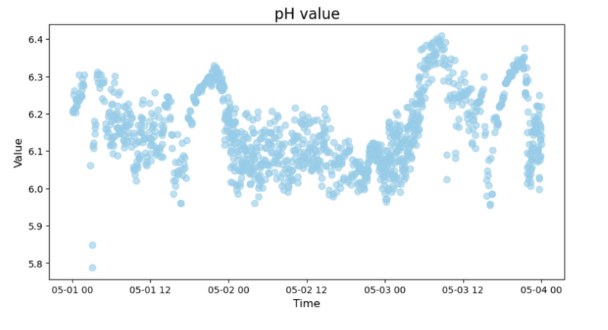
\includegraphics[width=0.8\textwidth]{Latex_Proposal/images/pH_graph.png} % 이미지 파일 이름
    \caption{pH Graph}
    \label{fig:pH_graph}
    \end{figure}

    \subsubsection{카메라 데이터}

    \paragraph{} 카메라 데이터의 경우 에어팜 내부 전체를 비추는 각도로, 1시간마다 snapshot을 찍어 base64형태로 cloud 저장소에 저장된다. 카메라 시선으로 3층 개체는 식물의 측면이 주로 보이고, 2층 개체는 식물의 윗면,1층 개체는 거의 보이지 않는다. 이러한 카메라 각도로 인해 식물이 가려져 팁번을 관찰하기 어려운 부분이 있다. 
    
    \begin{figure}[h]
    \centering
    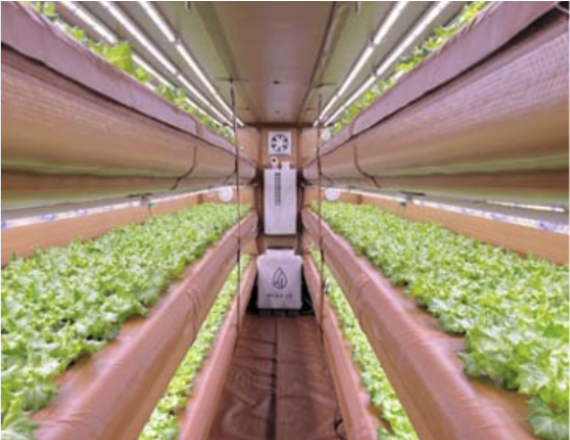
\includegraphics[width=0.5\textwidth]{Latex_Proposal/images/camera_view.png} % 이미지 파일 이름
    \caption{Camera View}
    \label{fig:camera_view}
    \end{figure}

    
    \subsection{Data pre-processing}
    \subsubsection{센서 데이터}
    \paragraph{} 센서 데이터는 시계열 데이터이기 때문에, N/A값을 삭제하기 보다는 임의적인 값으로 채우는 것이 데이터 분석에 유리할 것이다. 동일한 상수 값으로 채우거나, 앞/뒤 값과 동일하게 채우는 등 다양한 방법이 있지만 주변의 가까운 점으로부터 선형으로 결합된 가중치를 사용하는 보간법(interpolation)을 활용할 예정이다. 

    \paragraph{} 기존 미드바르에서 사용중인 이상값의 기준을 참고하여, 식물이 잘 자라지 않았거나 죽었을 때 기록된 센서 정보를 이상값으로 정의한다. 하지만 대부분의 경우 식물이 잘 자라기 때문에 이상값보다 정상값을 가지는 데이터가 훨씬 많을 것이다. 이렇게 데이터 불균형 문제가 발생했을 때 해결할 수 있는 방법으로는 resampling(over sampling, down sampling), 데이터 합성 등이 있다. resampling은 정상 데이터에서 샘플링 하여 개수를 줄이거나, 이상 데이터를 증강하여 정상 데이터와 이상 데이터의 양을 비슷하게 맞추는 것이다. 데이터 합성은 이상 데이터의 최근접 이웃을 이용하여 소수 데이터의 특성을 반영해 새로운 값을 만들어낸다. 하지만 데이터 합성은 기존의 이상 데이터를 기반으로 만들어지기 때문에 새로운 데이터에 취약할 수 있어 resampling을 사용할 예정이다\citep{bouarourou2023predictive}.

    \subsubsection{카메라 데이터}

    \paragraph{} 카메라 데이터는 개체를 하나하나 찍는 것이 아닌, 에어팜 전체를 찍는 카메라이기 때문에 전처리가 필수적이다. 한시간에 한번 snapshot으로 사진이 찍히는데, 사진이 찍히는 시간에 사람이나 다른 기구가 같이 나오거나, 전등이 꺼지는 시간에는 화면에 아무것도 나오지 않는 상황도 발생한다. 아래 사진과 같이 바로 사용하기 힘든 카메라 데이터는 필터 조정 등이 필요하다. 또한 전체 카메라 시선에는 식물이 자라는 1~3층 선반, 문, 환풍기, 밧줄 등이 모두 포함되기 때문에 이를 제거하고 식물 개체별로 볼 수 있도록 처리해야 한다. 그리고 카메라에서 먼 개체일수록 크기가 작게 나타나기 때문에 동일한 데이터 특성을 가질 수 있도록 처리도 필요하다. 

    \begin{figure}[h]
    \centering
    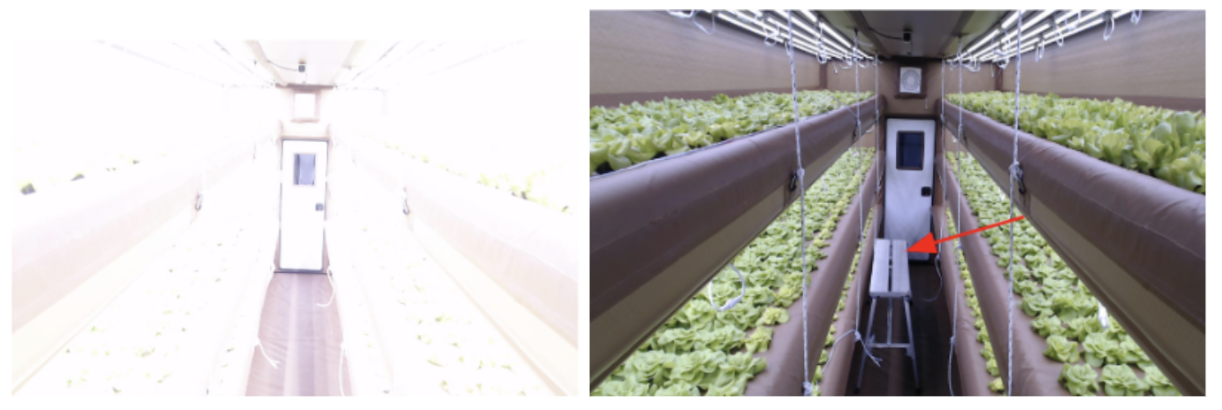
\includegraphics[width=0.9\textwidth]{Latex_Proposal/images/cam_pre.png} % 이미지 파일 이름
    \caption{Camera Data Preprocessing}
    \label{fig:came_pre}
    \end{figure}

    \paragraph{} 또한 팁번의 경우 식물 잎이 갈변하는 증상을 나타내기 때문에, 식물의 초록색과 팁번의 색이 명확히 대비된다. 이때 이미지 자체에 여러가지 필터를 적용하여 팁번이 더 잘 도드라지도록 전처리 할 수 있다. 그리고 센서데이터와 비슷하게 팁번이 발생한 개체 수가 정상 식물 개체수보다 훨씬 적기 때문에, 동일하게 데이터 불균형 문제가 발생한다. 이는 앞서 센서데이터 섹션에서 설명했던 resampling을 사용하거나 팁번 데이터를 증강하는 방법을 사용할 수 있는데, 이미지의 경우 생성형 AI를 이용하여 새로운 데이터를 생성할 수 있다. 이미지 필터 적용과 팁번 데이터 증강에 대해서는 method 섹션에서 더 자세히 설명할 예정이다. 


    \subsection{Data management}
    \begin{itemize}
    \item {공용서버 이용 및 데이터베이스 운영} \\
    주요 데이터를 공용서버에 저장하여, 팀원 모두가 데이터에 접근하고 관리할 수 있도록 할 예정이다. 또한 데이터 손실을 방지하고 원활하게 데이터를 꺼내올 수 있도록 데이터베이스를 운영할 예정이다.

    \item {정기적 백업} \\
    시스템 고장이나 데이터 손상시를 대비하여, 포터블 하드드라이브를 이용해 정기적인 백업을 진행할 예정이다. 주요 서버와는 분리된 다른 물리적인 위치에 보관함으로써 데이터를 안전하게 보관/유지할 수 있다.

    \item {자체적인 시스템 운영} \\
    공용서버와 물리적 백업 외에도, 미드바르가 운영하는 클라우드 시스템과 독립적인 소규모 시스템을 운영할 것이다. 이를 통해 주기적으로 최신 데이터를 업데이트 하고, 데이터 관리 효율성을 높일 수 있다.
    \end{itemize}

    \section{Method}                       
    \subsection{Methodologies}                       
    \subsubsection{센서 데이터}

    \paragraph {} 데이터 전처리를 완료한 후에는, 전통적인 이상감지 알고리즘을 적용해볼 수 있다. 이상 감지 알고리즘은 크게 분류하여 probability-based, distance-based, outlier ensembles 3개의 카테고리가 있다. 각각의 카테고리별로 해당하는 알고리즘을 간략하게 아래와 같이 설명할 수 있다\citep{de2020detecting}.
    
    \begin{enumerate}
        \item {Probability-based}
        \begin{itemize}
            \item {Angle-Based Outlier Detection (ABOD)} \\
            각 점들사이의 각도의 분산를 계산하여 이상값을 감지한다. 거리 기반 알고리즘이 잘 풀지 못하는 고차원 데이터에서 활용하면 효과적이다.
        \end{itemize}
    
        \item {Distance-Based}
        \begin{itemize}
            \item {Local Outlier Factor (LOF)} \\
            주어진 데이터 포인트와 이웃 점들간의 density deviation을 계산한다. 만약 주변의 점보다 압도적으로 낮은 밀도를 가진다면 이상값으로 간주한다.
            \item {K-Nearest Neighbors (KNN)} \\
            점들간의 거리를 계산하고, k개의 이웃 점들을 정의한다. 이웃 점들과 너무 멀리 떨어진 점일 수록 이상값으로 간주한다.
            \item {Cluster-Based Local Outlier Factor (CBLOF)} \\
            해당하는 점과 가장 가까운 cluster와의 거리를 계산한다. 아무 cluster에도 속하지 않거나 거리가 멀다면 이상값으로 간주한다.
        \end{itemize}
    
        \item {Outlier Ensembles}
        \begin{itemize}
            \item {Isolation Forest (iForest)} \\
            랜덤으로 feature와 split을 선택하여 random forest 알고리즘을 적용한다. 이 때 split의 수가 적을 수록 이상값으로 간주한다.
        \end{itemize}
    \end{enumerate}

    \paragraph {} 각 센서 데이터 그래프의 양상에 따라 다른 알고리즘을 적용할 수 있다. 한 예시로 아래와 같은 water temperature 그래프에서, 5월 3일부터 그래프의 밀도가 이전보다 높아지는 것을 확인할 수 있다. 이런 양상은 센서 값이 정상적인 패턴에서 벗어난 것을 의미한다. 따라서 해당 그래프에서는 density-based outlier detector중에 하나인 local outlier factor(LOF)를 사용할 수 있다. LOF는 데이터 포인트의 밀도를 기반으로 이상치를 탐지하는 알고리즘으로, 밀도가 다른 주변 데이터 포인트와 비교하여 현저히 낮은 포인트를 이상치로 식별한다. 이를 통해 데이터 포인트 간의 밀도 차이를 효과적으로 분석할 수 있으며, 밀도가 높은 구간에서도 이상치를 탐지할 수 있다.

    \begin{figure}[h]
    \centering
    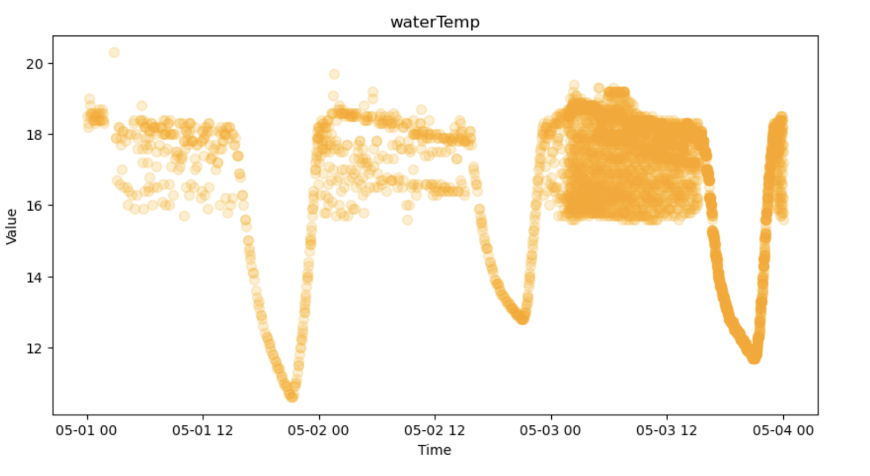
\includegraphics[width=0.8\textwidth]{Latex_Proposal/images/water_temperature_graph.png} % 이미지 파일 이름
    \caption{Water Temperature Graph }
    \label{fig:water_temp_graph}
    \end{figure}

    \paragraph   {} 하지만 전통적인 이상 감지 알고리즘은 데이터 각각의 “값" 을 기준으로만 이상 값을 탐지한다. 이를 보완하여 데이터의 “패턴" 을 인식함으로 이상값을 찾아내는 autoencoder또한 적용할 수 있다\citep{adkisson2021autoencoder}. Autoencoder는 신경망(Neural Network)을 기반으로 동작하는 딥러닝 기술로, 입력 데이터에서 중요한 패턴을 학습하고, 이를 바탕으로 데이터를 재구성함으로써, 이 과정에서 핵심 패턴을 추출하여 이상값을 감지하는 데 유용하다. Autoencoder는 비선형 변환을 통해 복잡한 패턴을 학습할 수 있으며, 이는 단순한 통계적 방법이나 거리 기반 방법보다 더 정교하게 이상값을 감지할 수 있다. 또한 하나의 센서 데이터 뿐만 아니라, 여러 종류의 데이터를 그래프에 한번에 나타내고, 복합적인 패턴을 학습하여 동시다발적으로 발생하는 이상현상의 징조를 알아낼 수 있다. 동종, 이종, 복합 상호테스트를 통한 감지로 센서 데이터를 종합 분석하여 고장을 효과적으로 감지할 수 있다\citep{lin2018sensortalk}.


    \subsubsection{카메라 데이터}
    
    \begin{enumerate}
        \item {Image filter (전통적인 Computer Vision)} 
    \paragraph{} 모델의 성능을 높이기 위해 전통적인 컴퓨터 비전 기법을 사용하여 팁번이 있는 영역을 더 확실하게 표시하고 빛이 반사되는 부분을 제거한다. 질병 부분에 해당하는 색상과 채도의 범위를 설정하고 그 범위에 해당하는 픽셀을 Binary Mask로 변환하여 생성할 수 있다. 

    \paragraph{} 이미지 전처리의 경우 이미지의 밝기 변화를 보정하여 정반사 부분을 제거하는 과정을 거친다. 가장 팁번이 많이 발생한 날짜를 기준으로 RGB 평균값을 얻어 그 값을 임계값으로 설정한다\citep{__2022}. Mean Shift Segmentation을 이용하여 식물의 이미지를 동일한 색상을 띠는 질병 부분을 하나의 클러스터로 그룹화하여 분할한다. HSV Color Segmentation을 활용하여 위 단계의 이미지를 HSV 색 공간으로 변환한다. 이를 통해 질병 부분에 해당하는 색상과 채도의 범위를 설정하고 그 범위에 해당하는 픽셀을 Binary Mask로 변환하여 생성한다.

        \item {WGAN}
    \paragraph{} 팁번에 해당하는 클래스의 경우 밀집된 곳에서 잘 보이지 않으므로 이미지를 통해 탐지하기가 어렵다. 팁번을 포함한 데이터가 불균형하게 분포된 현상이 발생할 수 있다\citep{gozzovelli2021tip}. WGAN 기반 데이터 증강을 통해 샘플과 비슷한 고품질의 이미지 생성이 가능하다. WGAN은 요즘 떠오르는 생성형 AI로, 이 알고리즘을 사용하면 팁번이 있는 데이터를 대량으로 만들어낼 수 있다.

    
    GAN은 데이터셋에서 합성 샘플 생성을 위해 널리 사용되는 기법이고, 이 GAN에서 실제 이미지와 생성된 이미지 분포 간의 이동 거리를 측정하는 것이 WGAN이다.

        \item {Anomaly Detection}
    
    \paragraph{} 이상 탐지에는 세 가지 접근법이 있다. 첫째, 이미지 전체를 하나의 클래스로 할당하는 분류(Classification)이다. 예를 들어, 이 이미지는 팁번인가 정상인가를 판단하는 것이다. 둘째, 이미지 내 여러 객체를 식별하고 위치를 지정하는 객체 탐지(Object Detection)이다. 여기서는 이미지 내 팁번의 위치를 찾는 작업이 포함된다. 셋째, 이미지의 각 픽셀을 클래스에 할당하여 객체의 형태를 정확히 파악하는 세분화(Segmentation)이다. 이를 통해 이미지 내 팁번의 정확한 형태를 식별할 수 있다\citep{liu2021plant}. 


    \paragraph{} 우리는 이 중에서 객체 탐지를 개발할 것이다. 분류는 한 이미지에 다량의 식물이 포함되어 있을 때 팁번의 유무만 확인하면 팁번을 찾는 데 많은 시간이 소요되기 때문이다. 세분화는 우리의 목표에 비해 시간적 및 인적 비용이 지나치게 많이 들기 때문에, 객체 탐지가 우리의 목적에 가장 적합하다고 판단했다.

        \item {Image Object Detection}
    \subparagraph{1)} 1-Stage Detector \\
    1-stage Detector는 Region Proposal과 Detection을 동시에 수행하는 방법으로, 대표적인 모형으로는 YOLO(You Only Look Once)와 SSD(Single Shot MultiBox Detector) 계열이 있다.

    \begin{itemize}
        \item {YOLO (You Only Look Once)는 이미지 전체를 한 번에 처리하여 객체를 탐지한다. YOLO는 네트워크를 단 한 번 통과시켜서 객체의 위치와 클래스 확률을 예측하기 때문에 매우 빠르다. 그러나 빠른 속도 때문에 작은 객체나 복잡한 장면에서의 정확도가 상대적으로 떨어질 수 있다.}

        \item {SSD (Single Shot MultiBox Detector)는 이미지의 여러 크기와 비율에서 물체를 탐지하기 위해 다양한 특징 맵에서 물체를 예측한다. 다양한 스케일에서 예측을 수행하여 작은 객체도 비교적 잘 탐지할 수 있으며, 여전히 1-stage 모델로서 빠른 속도를 유지한다.}
    \end{itemize}

    1-stage Detector는 속도가 빠르지만 정확도가 떨어질 수 있다는 특징이 있다. 그러나 실시간 처리가 중요한 자율 주행 및 다양한 실시간 애플리케이션에서 많이 사용된다.

    \subparagraph{2)} 2-Stage Detector \\
    2-stage Detector는 Region Proposal과 Detection을 순차적으로 수행하는 방법으로, 대표적인 모형으로는 R-CNN 계열이 있다 \citep{park20244}.
    
    \begin{itemize}
        \item {R-CNN (Regions with Convolutional Neural Networks)는 이미지에서 후보 영역을 제안(Region Proposal)하고, 이 후보 영역을 CNN을 통해 분류하는 방식이다. 기본 R-CNN은 매우 느리지만 높은 정확도를 가진다.}

        \item {Fast R-CNN는 R-CNN의 개선된 버전으로, 한 번의 CNN 연산으로 모든 후보 영역을 처리하여 속도를 향상시켰다. 또한, ROI Pooling을 도입하여 네트워크의 효율성을 높였다.}

        \item {Faster R-CNN은 Region Proposal Network(RPN)을 사용하여 후보 영역을 제안하는 단계를 CNN 안에 포함시켜 속도를 크게 개선하였다. 여전히 높은 정확도를 유지하면서도 이전 R-CNN보다 훨씬 빠르다.}
    \end{itemize}

    \paragraph{} 2-stage Detector는 순차적으로 수행하기 때문에 연산량이 많아 속도는 느리지만, 정확도가 높아 정밀한 객체 탐지가 필요한 응용 분야에서 많이 사용된다. 이번 연구에서는 2-stage Detector를 활용할 예정이다. 팁번을 탐지하는 데 있어 속도보다는 정확도가 중요하므로, 2-stage Detector의 뛰어난 정확도를 통해 팁번 탐지의 신뢰성을 향상시키고자 한다. 또한 한 이미지에 다량의 개체가 포함되어 있는 경우, 하나의 이미지를 여러개로 쪼개어 탐지할 식물의 수를 줄인 뒤에, 2-stage detector를 사용하는 것이 가능하다. 탐지 한 후에는 쪼개었던 이미지를 다시 원본 이미지와 같게 합성하여 팁번을 더 정확하게 탐지할 수 있다\citep{franchetti2022detection}.

     \end{enumerate}

    \subsection{Analytic process}
    \begin{enumerate}
    \item \textbf{데이터 수집 (Data collection)}: 미드바르 측에 요청하여 특정한 기간 동안의 센서데이터와 카메라 데이터를 수집한다.
    \item \textbf{데이터 탐색 (Data exploration)}: 시각화 도구를 사용하여 데이터의 패턴과 트렌드를 파악한다. 히스토그램, 산점도, 박스 플롯 등을 활용할 수 있다.
    \item \textbf{데이터 전처리 (Data preprocessing)}: 결측값을 제거, 이상값을 레이블링, 데이터 정규화 등을 수행한다.
    \item \textbf{이상탐지 (Anomaly Detection)}: 데이터의 특성과 분석 목적에 맞는 이상 감지 알고리즘을 선택하여 적용한다.
    \item \textbf{시각화 (Visualization)}: 이상 감지 결과를 이해하기 쉽도록 시각화한다. 이상값의 위치를 직접 표시하여 그래프를 그릴 수 있다.
    \item \textbf{평가 (Evaluation)}: 성능을 평가하고, 다양한 평가 지표를 통해 피드백을 수집한다.
\end{enumerate}




    \subsection{Validation strategy}
    \begin{itemize}

    \item {결과 검증 } 
    
    모델의 결과가 실제 상황과 일치하는지 확인한다. 해당 데이터 전문가(미드바르 재배팀 혹은 소프트웨어 팀)의 의견을 반영하여 결과의 타당성을 검증한다. 또한 다양한 시나리오를 설정하여 모델의 반응을 테스트하고, 예측한 이상값이 실제로 의미있는지 평가한다.

    \item {피드백 수집 및 반복 개선}  
    
    분석 결과를 미드바르 팀에 공유하고 피드백을 수집한다. 이를 바탕으로 데이터 전처리, 모델 선택 및 학습, 평가 단계를 반복하여 모델의 성능을 지속적으로 향상시킨다.
    \end{itemize}

    \section{Expected results}   
    \subsection{센서 데이터} 

    \paragraph{} 이상 값을 그래프에 표시해줌으로써 대시보드를 통해 이상값이 발생했음을 확인할 수 있다. 
    \begin{figure}[h]
    \centering
    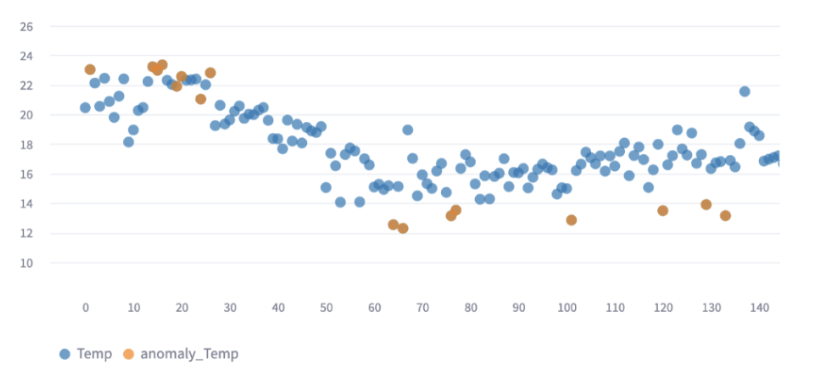
\includegraphics[width=0.8\textwidth]{Latex_Proposal/images/sensor_ex.png} % 이미지 파일 이름
    \caption{Anomaly Detection of Sensor Data }
    \label{fig:sensor_ex}
    \end{figure}


    \subsection{카메라 데이터} 
    \paragraph{} 카메라 화면에 직접 bounding box로 팁번의 위치를 표기함으로써 데이터가 전송되는 즉시 팁번 발생 여부를 확인할 수 있다. 

    \begin{figure}[h]
    \centering
    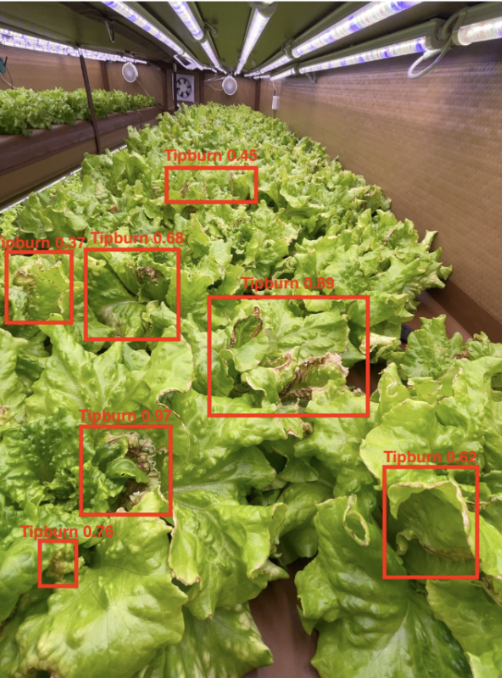
\includegraphics[width=0.3\textwidth]{Latex_Proposal/images/tipburn_ex.png} % 이미지 파일 이름
    \caption{Anomaly Detection of Camera Data }
    \label{fig:tipburn_ex}
    \end{figure}

    \pagebreak
    
    \bibliographystyle{apalike} % apalike 
    \bibliography{proposal_bib}

\end{document}
